% Section content template for individual Educative lessons
% This file contains the actual content for a specific section
% Generated from Educative API section content

% Section: Introduction to Databases
% Section ID: 4901035478351872
% Section Slug: introduction-to-databases
% Generated: 2025-12-06T21:13:58.042190

\subsection{Problem statement}\label{wzCjoc6XwGctsAx5SdhtK}
\\
Let's start with a simple question. Can we make a software application without using databases? Let's suppose we have an application like WhatsApp. People use our application to communicate with their friends. Now , where and how can we store information (a list of people's names and their respective messages) permanently and retrieve it?
\\
We can use a simple file to store all the records on separate lines and retrieve them from the same file. But using a file for storage has some limitations.

\subsubsection{Limitations of file storage}\label{cXRi4Y7PVc-xNrbdvE8YZ}

\begin{itemize}
\item
\protect\phantomsection\label{6HUKF2wTkK-7wpR7boFGM}
We can't offer concurrent management to separate users accessing the storage files from different locations.
\item
\protect\phantomsection\label{bvaU3x-_-jZ8KCHfDVACv}
We can't grant different access rights to different users.
\item
\protect\phantomsection\label{hfPHrQ2OW9Lpzw7Y4jl_X}
How will the system scale and be available when adding thousands of entries?
\item
\protect\phantomsection\label{GnyuGua5GavQGv5eHCfnD}
How will we search content for different users in a short time?
\end{itemize}

\begin{figure}[htbp]
 \centering
 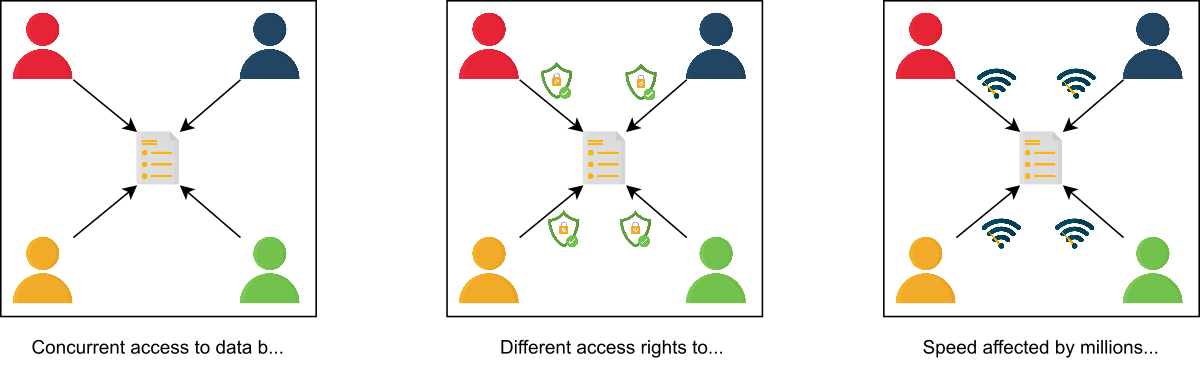
\includegraphics[width=0.5\textwidth]{Images/chapter_9/section_4901035478351872/5143892395819008.png}
 \caption{The limitations of file storage}
\end{figure}

\subsubsection{Solution}\label{hB5zpiPg1pGnY_ffCJiMd}
\\
The above limitations can be addressed using databases.
\\
A \textbf{database} is an organized collection of data that can be managed and accessed easily. Databases are created to make it easier to store, retrieve, modify, and delete data in connection with different data-processing procedures.

\begin{figure}[htbp]
 \centering
 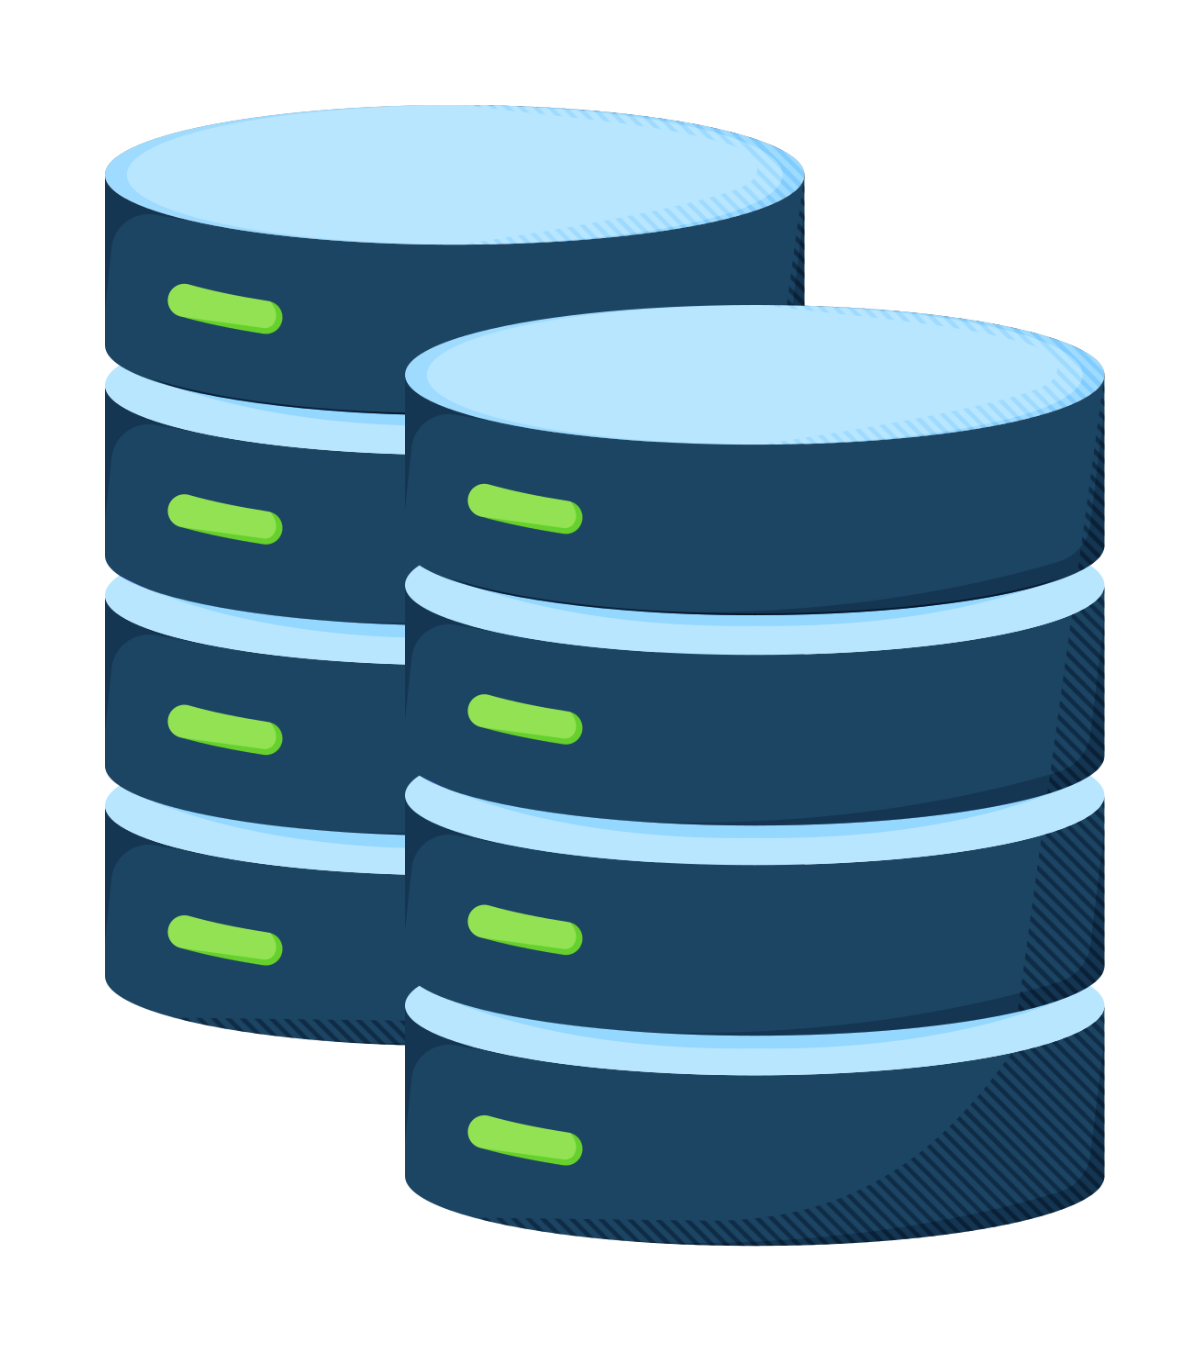
\includegraphics[width=0.25\textwidth]{Images/chapter_9/section_4901035478351872/4603635655639040.png}
 
\end{figure}

Some of the applications where we use database management are the banking systems, online shopping stores, and so on. Different organizations have different sizes of databases according to their needs.
\begin{quote}
\textbf{Note}: According to a source, the World Data Center for Climate (WDCC) is the largest database in the world. It contains around 220 terabytes of web data and 6 petabytes of additional data.
\end{quote}
\\
There are two basic types of databases:

\begin{itemize}
\item
\protect\phantomsection\label{b-q_EC8egN6QYRpNPXu0n}
SQL (relational databases)
\item
\protect\phantomsection\label{wfQi-0ZvBztmj9eyIJwxv}
NoSQL (non-relational databases)
\end{itemize}
\\
They differ in terms of their intended use case, the type of information they hold, and the storage method they employ.

\begin{figure}[htbp]
 \centering
 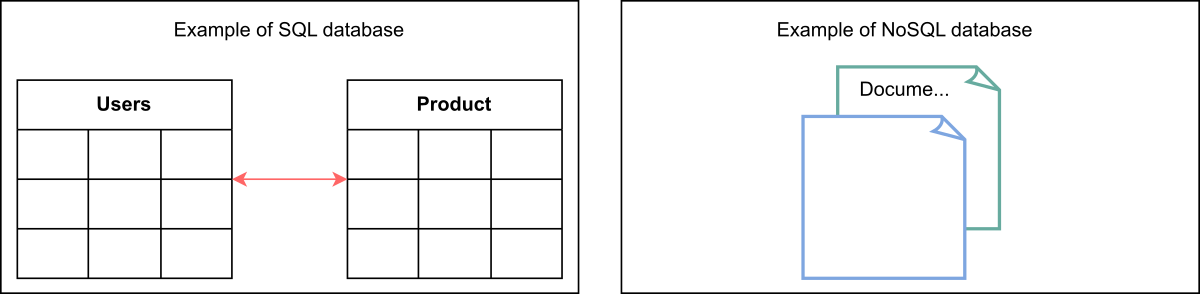
\includegraphics[width=0.5\textwidth]{Images/chapter_9/section_4901035478351872/5042637977157632.png}
 \caption{Relational database has a well defined structure such as attributes (columns of the table). NoSQL databases such as document databases often have application-defined structure of data.}
\end{figure}

Relational databases, like phone books that record contact numbers and addresses, are organized and have predetermined schemas. Non -relational databases, like file directories that store anything from a person's contact information to shopping preferences, are unstructured, scattered, and feature a dynamic schema. We
'll discuss their differences and their types in detail in the next lesson.

\subsection{Advantages}\label{1ZKn6rFtnPb7hDnxhY9__}
\\
A proper database is essential for every business or organization. This is because the database stores all essential information about the organization, such as personnel records, transactions, salary information, and so on. The following are some of the reasons why the database is important:

\begin{itemize}
\item
\protect\phantomsection\label{-LWDdjvLLR7kRwssOOfk4}
\textbf{Managing large data}: A large amount of data can be easily handled with a database, which wouldn't be possible using other tools.
\item
\protect\phantomsection\label{6vm3aqgt0TnSQvrFmG7_J}
\textbf{Retrieving accurate data (data consistency)}: Due to different constraints in databases, we can retrieve accurate data whenever we want.
\item
\protect\phantomsection\label{JluO0mYdN9n8FOFrggeVO}
\textbf{Easy updation}: It is quite easy to update data in databases using data manipulation language (DML).
\item
\protect\phantomsection\label{zVIOKorKR8-aySV1EQ2Po}
\textbf{Security}: Databases ensure the security of the data. A database only allows authorized users to access data.
\item
\protect\phantomsection\label{AopAHE66MHfQZPO0BF6me}
\textbf{Data integrity}: Databases ensure data integrity by using different constraints for data.
\item
\protect\phantomsection\label{QDELUSsE1LQT1hSLYsslx}
\textbf{Availability}: Databases can be replicated (using \href{https://www.educative.io/courses/grokking-the-system-design-interview/data-replication}{data replication}) on different servers, which can be concurrently updated. These replicas ensure availability.
\item
\protect\phantomsection\label{KZ8Xd7eoEfpLm38jCz1Ky}
\textbf{Scalability}: Databases are divided (using \href{https://www.educative.io/courses/grokking-the-system-design-interview/data-partitioning}{data partitioning}) to manage the load on a single node. This increases scalability.
\end{itemize}

\subsection{How will we explain databases?}\label{T0U_5IqKBYBmnWTMATD7e}
\\
We have divided the database chapter into four lessons:

\begin{enumerate}
\item
\protect\phantomsection\label{Ff_enAWEJeDLUhNh6gitD}
\href{https://www.educative.io/courses/grokking-the-system-design-interview/types-of-databases}{\textbf{Types of Databases}}: We'll discuss the different types of databases, their advantages, and their disadvantages.
\item
\protect\phantomsection\label{yKINSzyLWuKsCdmxB74q9}
\href{https://www.educative.io/courses/grokking-the-system-design-interview/data-replication}{\textbf{Data Replication}}: We'll discuss what data replication is and its different models with their pros and cons.
\item
\protect\phantomsection\label{iAykAHt3UqpjtA8miUPum}
\href{https://www.educative.io/courses/grokking-the-system-design-interview/data-partitioning}{\textbf{Data Partitioning}}: We'll discuss what data partitioning is and its different models with their pros and cons.
\item
\protect\phantomsection\label{_KvPaWf568kg4DsfjxrMi}
\href{https://www.educative.io/courses/grokking-the-system-design-interview/trade-offs-in-databases}{\textbf{Cost-benefit analysis}}: We'll discuss which database sharding approach is best for different kinds of databases.
\end{enumerate}
\\
Let's get started by understanding different types of databases and their preferred use cases.

% End of section content